\chapter{Analysis Process and Result}

The Lyapunov function approach require 3 components which forms the optimzation problem described in chapter 3 to produce a worst-case performance convergence rate: the state update matrices, the constraints formed by the interpolation conditions and the performance measure. These components are derived from the input provided to JuPE which undergo transformations before they can be used to create an optimization problem in the JuMP modelling language, the process of which can be described in 3 steps:
\begin{enumerate}
    \item JuPE automatically uses the input provided to form a systematic charaterization the analysis problem using data structures described in chapter 4, including how the algorithm being analyzed updates, the constraints created by the interpolation conditions of the class of function and the performance measure.
    \item These data structures are converted to real number vectors and matrices that represent the updated state of the algorithm and each algorithm in the form of the a linear function of the initial states and inputs.
    \item An optimization problem is created inside a JuMP model using these representations and solved to verify whether a certain convergence rate is feasible for a given problem. This process is repeated with different convergence rates as JuPE search for the lowest feasible convergence rate.
\end{enumerate}

This chapter details the analysis process, including how these steps are performed for component and how the optmization problem is formed and solved to derive worst-case performancce convergence rate. In addition, the analysis result of three algorithms over smooth strongly convex functions will also be detailed as an example of the result produced by algorithm analysis.

\subsection*{Real scalars and linear form}

% In JuPE, when variable expressions are defined in an inner product space, they are vector. These expressions include states of an algorithm, the starting and end points, and the gradient of a function at a point. This is because a function class is multidimensional, which means each point or iterate is a vector whose size is identical to the dimension of the function. 

All three components needed to form the linear matrix inequality - the Lyapunov functions $V(x_k)$ and $V(x_{k+1})$ and the left hand side of each constraint - from equations \ref{eqn:int_cond2}, \ref{eqn:Ly_ineq} and \ref{eqn:Ly_ineq2} are functions linear in the elements of the Gram matrix and optimization variables. On the other hand, the JuMP modeling language does not support the expression and constraint data structures presented in chapter 4, and the LMIs of \ref{Ly_ineq2} must be transformed into a function linear in the optimization variables and real numbers before it can be formed inside the JuMP model. JuPE achieve this by creating a vector of every elements of the Gram matrix and expressing every component that forms the LMIs as a linear function of this vector. This process is done in three steps, which are:
\begin{enumerate}
    \item Of every expressions that has been created during the input process, define the initial state vector x as every real expressions which contain another expression in its next field.
\begin{figure}[h!]
    \begin{lstlisting}[mathescape]
x  = collect(v for v $\in $ vars if !ismissing(next(v)) && v isa R)
4-element Vector{R}:
    |x0|$^2$
    |xs|$^2$
    <x0,xs>
    <xs,x0>
\end{lstlisting}
\caption{Initial state real scalar expressions from example \ref{ex_analysis}}
\label{ex_initstate}
\end{figure}

    \item Define an update state vector x$^+$ consisting of the next expression of every expression in the initial state. The input vector u is then defined as every real expression that exist in the decomposition of the updated state expressions but not in the initial state expressions.
    \begin{figure}[h!]
        \begin{lstlisting}[mathescape]    
x$^+$ = next(x)
4-element Vector{R}:
    <x0,xs> - 0.18181818181818182 <$\nabla $f(x0),xs>
    -0.18181818181818182 <$\nabla $f(x0),x0> + 0.03305785123966942 |$\nabla $f(x0)|$^2$ - 0.18181818181818182 <x0,$\nabla $f(x0)> + |x0|$^2$
    -0.18181818181818182 <xs,$\nabla $f(x0)> + <xs,x0>
    |xs|$^2$

u  = collect(setdiff(variables(x$^+$), variables(x)))
5-element Vector{Expression}:
    <xs,$\nabla $f(x0)>
    <x0,$\nabla $f(x0)>
    <$\nabla $f(x0),xs>
    <$\nabla $f(x0),x0>
    |$\nabla $f(x0)|$^2$
        \end{lstlisting}    
    \caption{Updated state and input real scalar expressions from example \ref{ex_analysis}}
    \label{ex_updatedstate_input}
    \end{figure}
    \item The initial state and input vector [x; u] can now form every expression in the optimization problem, which means any real scalar expression can be transformed into a linear function of [x; u] by finding the matrix or vector with which to multiply [x; u] to find that expression. This transformation, which will be refered to as the linear form of an expression, can be derived by finding the values of each expression in the initial and state input vector present in the expression's decomposition dictionary.
\end{enumerate}

\begin{figure}[h!]
    \begin{lstlisting}[mathescape] 
linear_form = vec(linearform([x; u] => x0^2 - 3*(x0'*xs)))
linear_form'*[x; u]
Scalar in R
  Decomposition: -3 <xs,x0> + |x0|$^2$
\end{lstlisting}    
\caption{Example of linear form of a scalar expression \ref{ex_analysis}}
\label{ex_linearform}
\end{figure}

\section{Performance measure}
The linear form matrix of the performance measure is the first of the three components needed to form the Lyapunov function ($||\xi _k - \xi _s||^2$ in \ref{eqn:Ly_ineq}). For example, the performance measure in \ref{ex_analysis}, which is defined as $(x0-xs)^2$ and which evaluates into $|x0|^2 - <xs, x0> - <x0, xs> + |xs|^2$, has the linear form:
\begin{figure}[h!]
\begin{lstlisting}[mathescape]
$\mathcal{P} $ = vec(linearform( [x; u] => performance ))
print($\mathcal{P}$)
[-1, -1, 1, 1, 0, 0, 0, 0, 0]
\end{lstlisting}
\caption{Linear form matrix of expression $(x0-xs)^2$}
\label{ex_linearform2}
\end{figure}

\section{Algorithm, state update and Lyapunov function formulation}
% \subsection*{State space matrix and their linear form formulation}
As shown in \ref{ex_analysis}, the algorithm to be analyzed is inputted into JuPE first by defining an initial state and how a 'next' state is updated from the initial state. The initial state is defined to be a vector in an inner product space, and the updated state is a linear function of one or multiple initial state and the gradient of the function evaluated at some point. While the gradient descent algorithm updates using only one state and evaluate the gradient at the previous state, if an algorithm updates using multiple past states or the gradient at an interpolated point, these vectors will also have to be defined.

The forming of the algorithm can then be completed by defining the relationship between states and their next states using the "=>" operation, which updates the next field of every expression in the decomposition of which there is the state on the left hand side of the operation.

\begin{figure}[h!]
	\begin{lstlisting}[mathescape]
next(x0)

Vector in R$^n$
  Label: x1
  Decomposition: -0.18181818181818182 $\nabla $f(x0) + x0
  Associations: Dual => x1*

next(x0'*xs)

  Scalar in R
    Decomposition: -0.18181818181818182 <xs,$ \nabla $f(x0)> + <xs,x0>
\end{lstlisting}
\caption{next field of a state vector expressions and a scalar formed from a state expression}
\label{ex_next}
\end{figure}

The initial and update state vectors are created in \ref{ex_initstate} and \ref{ex_updatedstate_input}, their linear form matrices is the second of the three components needed to formulate the Lyapunov function and can be formed as:

\begin{figure}[h!]
    \begin{lstlisting}[mathescape]
X  = linearform([x; u] => x)
    4x9 Matrix{Int64}:
    1  0  0  0  0  0  0  0  0
    0  1  0  0  0  0  0  0  0
    0  0  1  0  0  0  0  0  0
    0  0  0  1  0  0  0  0  0

X$^+$ = linearform([x; u] => x$^+$)
    4x9 Matrix{Real}:
    1  0  0  0   0          0         -0.181818  0           0
    0  1  0  0  -0.181818   0          0         0.0330579  -0.181818
    0  0  1  0   0         -0.181818   0         0           0
    0  0  0  1   0          0          0         0           0
    
    \end{lstlisting}
    \caption{Linear form state matrices x and x$^+$}
    \label{ex_linearform_state}
    \end{figure}

% \subsection*{State space in Lyapunov function}
Following the steps presented in chapter 3, the Lyapunov function can begin to be formed by first defining an optimization variable $P$ in the JuMP model as a JuMP variable. Once JuMP and the solver start optimizing the problem, P is one of the variable that will be optimized to produce a solution. The LMIs are then created as:

\begin{subequations} \label{eqn:Ly_ineq3}
	\begin{align}
	    L1 = \mathcal{P} - X^TP      \\
        L2 = X^{+T}P - \rho X^TP
	\end{align}
\end{subequations}

\section{Constraints}
As presented in 4.3, the oracle created from the class of function and the transpose of each expression automatically forms the interpolation condition and Gram matrix constraints. These constraints are linearized and added to the optimization in 2 steps:
\begin{description}
    \item [Optimization variable multipliers] For each constraint, two optimization variables $\lambda$ and $\mu$ are as JuMP variables. These variables are the $\lambda$ in \ref{eqn:int_cond2}. If the constraint is created from the interpolation condition for the transpose of state vectors and is applied to a matrix of real scalar expressions, the optimization variable will be a matrix sharing the same size with the matrix constrained. If the constraint is created from the interpolation conditions of the class of function and is applied to a single real scalar expression, the optimization problem created will have a size of 1.
    \item [Constraint on multiplier] The JuMP variables multipliers are constrained in the JuMP model depending on the constraint expression they were created for: The multiplier is not constrained if the expression is constrained to be zero, constrained to be non-negative if the expression is constrained to be non-negative, and constrained to be symmetrical and in the JuMP supported positive semidefinite cone if the expression is constrained to be positive semidefinite.
    \item [Linear form of constraints] The linear form of each constraint scaled by the multiplier is created and added to the Lyapunov functions.
\end{description}

If the expression constrained is a single real scalar, the linear form of the constraint is derived similarly to the linear form of the performance measure or state space matrices but scaled by the multiplier. Suppose we have the constraint $(x0 - xs)^2 \geq 0$ and matrix $\bmat{x\\ u} = \bmat{|x0|^2\\ <xs, x0>\\ |xs|^2}$, the linear form of the constraint in terms of $\bmat{x\\ u}$, denoted as $M$ would be:

\begin{subequations} \label{eqn:constraint_single}
	\begin{align}
    \lambda * (x0 - xs)^2 &= M * \bmat{|x0|^2\\ <xs, x0>\\ |xs|^2} \label{eq_cons_single1}       \\
	M &= \bmat{\lambda& 2\lambda & \lambda} \label{eq_cons_single2}
	\end{align}
\end{subequations}

If the expression constrained and its corresponding multiplier are vectors of expression, the linear form of the constraint is derived as the linear form of the inner product between the multiplier vector and the constraint expression vector. Suppose we have a constraint vector $\bmat{(x0-xs)^2 \\ (x0-xs)^2-3*|xs|^2} \geq 0$ and the same $\bmat{x\\ u}$ matrix as \ref{eqn:constraint_single}, the linear form of the constraint in terms of $\bmat{x\\ u}$, denoted as $M$ would be:

\begin{subequations} \label{eqn:constraint_vector}
	\begin{align}
    \bmat{\lambda  & \lambda } * \bmat{(x0 - xs)^2 \\ (x0 - xs)^2-3*|xs|^2} &= M * \bmat{|x0|^2\\ <xs, x0>\\ |xs|^2} \label{eq_cons_vector1}       \\
	M &= \bmat{\lambda & -\lambda & \lambda \\ \lambda & -\lambda & -2*\lambda} \label{eq_cons_vector2}
	\end{align}
\end{subequations}

And if the expression constrained and its corresponding multiplier are matrices, the linear form of the constraint is the linear form of the trace of the matrix multiplication between the multiplier and the constraint expression. For the Gram matrix in \ref{eqn:trans_cond} constrained to be positive semidefinite, its linear form would be:

\begin{equation} \label{eqn:trans_cond}
	tr(\lambda \bmat{||x0||^2 & \innerproduct{xs}{x0} & \innerproduct{\nabla f(x0)}{x0} \\ \innerproduct{x0}{xs} & ||xs||^2 & \innerproduct{\nabla f(x0)}{xs} \\ \innerproduct{x0}{\nabla f(x0)} & \innerproduct{xs}{\nabla f(x0)} & ||\nabla f(x0)||^2]}) \geq 0	
\end{equation}

Where $\lambda $ is a 3x3 JuMP variable. In all three cases, the resulting linear form matrix is the linear form of the constraint expression scaled by the JuMP variable multipliers. For each constraints, 2 linear form matrices are created and added to the two Lyapunov functions, completing the final LMIs

\section{Derived feasibility and bisection search}
Following equations \ref{eqn:Lyapunov} in section 3.3, the LMIs can now be solved: the solver of the JuMP model is called to optimize the problem and find the varibles $P$, $\lambda$ and $\mu$ for which the LMIs is satisfied, and a convergence rate $\rho$ can be guaranteed.

Due to the formulation of the Lyapunov functions, a convergence rate of 1 means the algorithm is not converging and a convergence rate of 0 means the algorithm converge after a single iterate. JuPE performs bisection search, also known as binary search, for the smallest value $\rho$ between 0 and 1 that makes the optimization problem feasible, calling performing the steps presented in this chapter for each value $\rho$ and checking feasibility at each iterate of the search. The smallest value $\rho$ found within a tolerance of $1E-5$ is returned as the guaranteed convergence rate, and the analysis process is complete.

\section{Result}
After running JuPE to perform algorithm analysis on 3 algorithms (GD), (HB), and (FG) on classes of m strong L smooth convex function where the condition number L/m are chosen between 1 and 10, we get 
\begin{figure}[h]
    \centering
    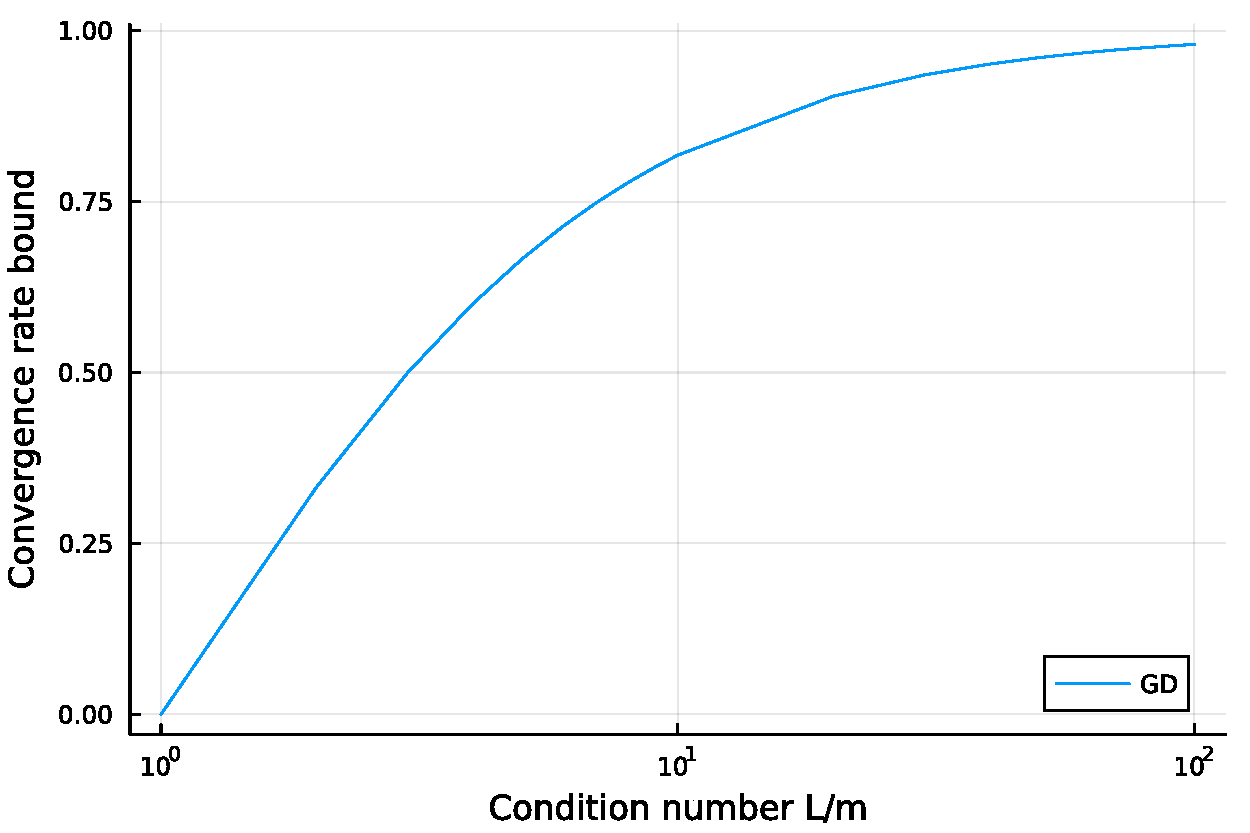
\includegraphics[width = .8 \textwidth]{plot.pdf}
    \caption{Convergence rate guarantee for 3 algorithms over m strong L smooth convex function}
    \label{plot_result}
\end{figure}